\documentclass[a4paper, 12pt]{article}

\def\languages{french, english}

%%%%%%%%%%%%%%%%%%% Libraries

\input{include/libraries/bibliography.tex}
\input{include/libraries/default.tex}
\input{include/libraries/figures.tex}
\input{include/libraries/informatics.tex}
\input{include/libraries/mathematics.tex}
\input{include/libraries/theorems.tex}
\input{include/libraries/units.tex}

\input{include/languages/french.tex}

%%%%%%%%%%%%%%%%%%% Titlepage

\def\logopath{resources/pdf/logo-uliege.pdf}
\def\toptitle{University of Liège}
\title{Motivation \& Control Problem}
\def\subtitle{Linear control systems}
%\def\authorhead{Author}
\author{
    Bastien \textsc{Hoffmann} (20161283)\\
    Maxime \textsc{Meurisse} (20161278)\\
    Valentin \textsc{Vermeylen} (20162864)\\
}
%\def\rightauthorhead{}
%\def\rightauthor{}
\def\context{Master in Civil Engineering}
\date{Academic year 2019-2020}

%%%%%%%%%%%%%%%%%%% Options

\fancyhead[R]{}
\renewcommand{\thesubsection}{\arabic{subsection}}
\addbibresource{references.bib}
\defbibheading{bibliography}[\refname]{}

%%%%%%%%%%%%%%%%%%% Document

\begin{document}
    % ----- Titlepage ----- %
    \input{include/titlepages/default.tex}
    
    % ----- Choice of the topic ----- %
    \subsection{Choice of the topic}
    The chosen topic is : {\bf Active mass damper}.
    
    % ----- Context ----- %
    \subsection{Context}
    The current engineering prowesses allow us to build buildings higher and higher. These constructions are subject to various disturbances (mainly wind, but also earthquakes) that make them oscillate. They turn into giant pendulum and swing from left to right, sometimes moving several meters at the top !\cite{YouTube_minutephysics}\par
    To reduce these oscillations, we use a passive system, called {\it tuned mass damper}, which consists of concealing a tuned and harmonic oscillator at the top of the tower. It is coupled to its movement and oscillates in phase opposition to recover the kinetic energy of the tower and thus reduce the oscillations.\cite{Wikipedia_amortisseur_tmd}\par
    An active version of this system exists : the {\it active mass damper}. It consists of the same principle as the tuned mass damper but it is equipped with sensors and actuators to measure the oscillations of its environment and, via an algorithm, generate a movement for the mass that reduce or totally remove these oscillations.\cite{sciencedirect_amd}\par
    Our study field focuses on the active mass damper systems used to reduce the oscillations caused by the {\bf wind} on {\bf tall} buildings. More specifically, we will focus on a simplified model : a block linked to a spring (to simulate the oscillations of the building) and a smaller moving mass placed over it that stabilises the system.\par
    This model is presented in figure \ref{fig:schema}.
    \begin{figure}[!ht]
        \centering
        \includegraphics[width=0.7\textwidth]{resources/pdf/schema.pdf}
        \caption{Simplified schema of an active mass damper for stabilise a tall building}
        \label{fig:schema}
    \end{figure}
    
    % ----- Control problem diagram ----- %
    \subsection{Control problem diagram}
    The diagram of our control problem is shown in figure \ref{fig:diagram}.
    \begin{figure}[!ht]
        \centering
        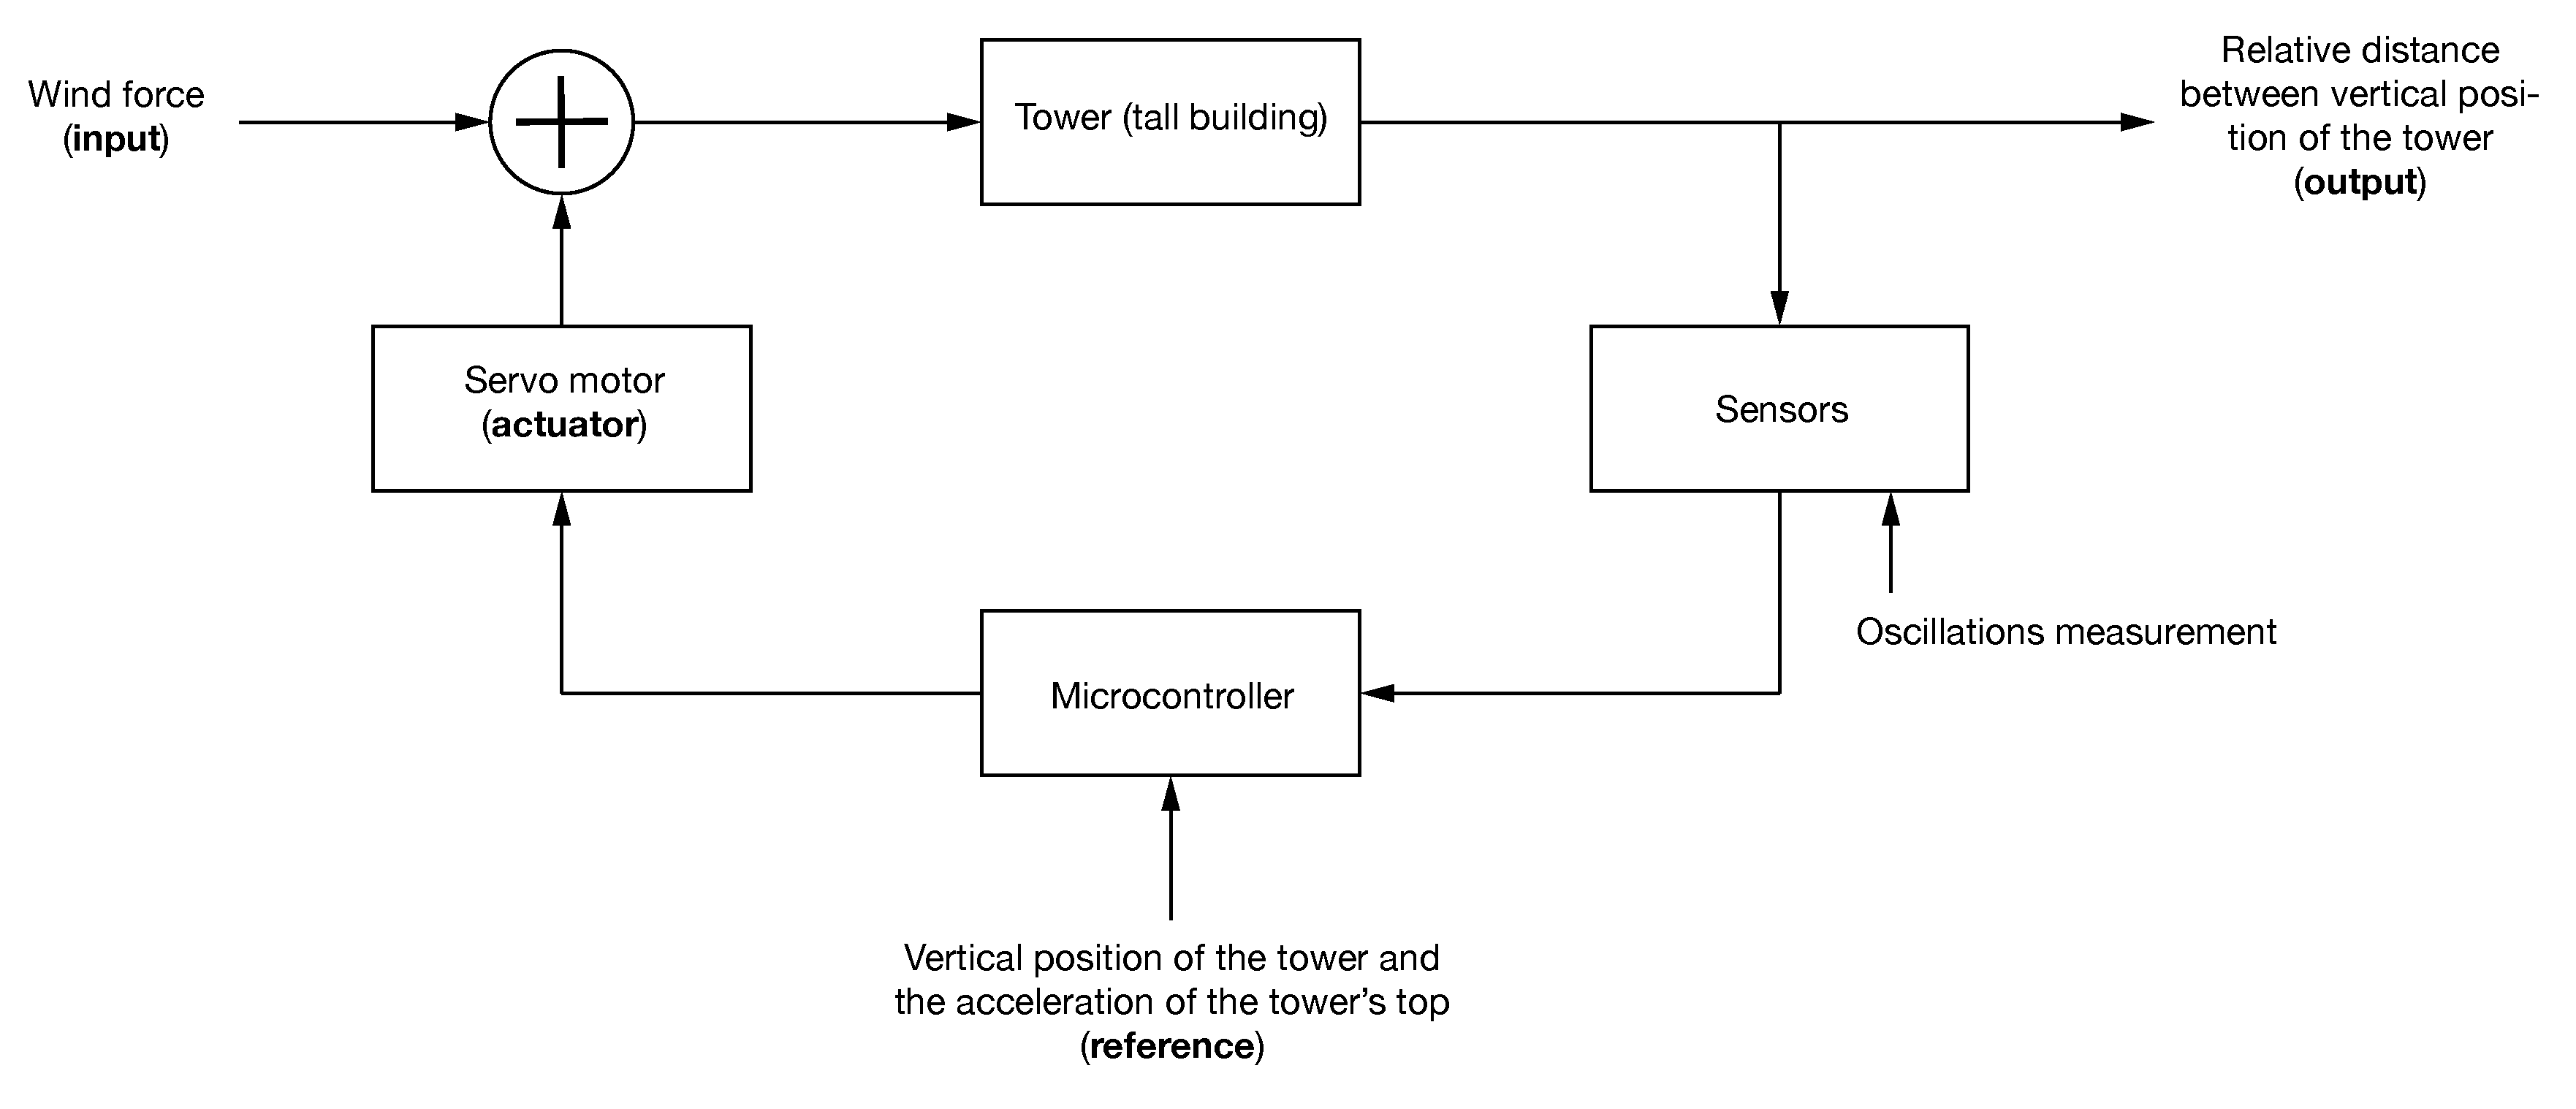
\includegraphics[width=1\textwidth]{resources/pdf/diagram.pdf}
        \caption{Control problem diagram of the active mass damper for tall buildings problem}
        \label{fig:diagram}
    \end{figure}
    
    % ----- Control problem description ----- %
    \subsection{Control problem description}
    \begin{itemize}
        \item {\bf Utility of the controller} : the controller allows the system to be active, {\it i.e.} to measure the oscillations to which it is subjected and to generate a movement, thanks to the servo-motor, for the moving mass that will reduce, or even eliminate totally, the oscillations.
        \item {\bf System to be controlled} : the tower, and more specifically its position.
        \item {\bf Inputs of the system} : wind forces acting on the tower and on the moving mass.
        \item {\bf Outputs of the system} : the relative distance between the vertical position and the displacement of the tower and the horizontal acceleration of the top of the tower relative to the ground.
        \item {\bf Reference} : the vertical position of the tower and an acceleration of \SI{0}{\meter\per\second\squared}.
        \item {\bf Actuators} : servo-motor to move the cart that reduces the oscillations.
        \item {\bf Constraints and limitations} : to simplify our system, we consider a tower \SI{500}{\meter} high, perfectly vertical when it undergoes no disturbance. The only disturbance on this tower is the strength of the wind. The wind, ranging from a few tens of \SI{}{\kilo\meter/\hour} to a hundred \SI{}{\kilo\meter/\hour}, can swing the tower from a few centimetres to several meters.
    \end{itemize}
    
    % ----- Reference ----- %
    \newpage
    \subsection{Reference}
    \nocite{*}
    \printbibliography
\end{document}
